\section{Classification Methods}


\subsection{Classification Problems and Decision Boundaries}


\begin{frame}{The Classification Problem}
    \begin{itemize}
        \item The response $y^{(i)}$ is qualitative: it takes one of $K$ classes, $y^{(i)} \in \{1, \dots, K\}$, or $y^{(i)} \in \{0, 1\}$ when $K = 2$.
        \item Training data: $\{(\mathbf{x}^{(i)}, y^{(i)})\}_{i=1}^{n}$ with feature vectors $\mathbf{x}^{(i)} = (x_1^{(i)}, \dots, x_p^{(i)})^\top \in \mathbb{R}^p$.
        \item Goal: learn a classifier $f : \mathbb{R}^p \to \{1, \dots, K\}$ such that $\hat{y}^\ast = f(\mathbf{x}^\ast)$ is correct for a new observation $\mathbf{x}^\ast$.
        \item Intercept notation: $\tilde{\mathbf{x}}^{(i)} = (1, \mathbf{x}^{(i)\top})^\top \in \mathbb{R}^{p+1}$ prepends a $1$, and the design matrix $\tilde{\mathbf{X}} \in \mathbb{R}^{n \times (p+1)}$ has rows $\tilde{\mathbf{x}}^{(i)\top}$. Coefficient vectors such as $\symbf{\beta} = (\beta_0, \beta_1, \dots, \beta_p)^\top$ include the intercept.
    \end{itemize}
\end{frame}


\begin{frame}{Classification vs.\ Regression}
    \begin{itemize}
        \item Regression predicts a quantitative response; classification predicts a category.
        \item Examples: spam vs.\ not spam, loan default, land-cover class from spectral bands, disease present vs.\ absent.
        \item Most classifiers first estimate a probability for each class, and then assign the observation to a class using these probabilities.
    \end{itemize}
\end{frame}


\begin{frame}{Why Not Linear Regression?}
    \begin{columns}[T]
        \begin{column}{0.48\textwidth}
            \begin{sitemize}
                \item Coding a binary response as $y^{(i)} \in \{0, 1\}$ and fitting $\hat{y} = \hat{\symbf{\beta}}^\top \tilde{\mathbf{x}}$ gives fitted values that are not confined to $[0, 1]$, so they are not valid probabilities.
                \item For $K > 2$, coding the classes as $1, 2, 3, \dots$ imposes an ordering and equal spacing that the classes do not have.
                \item We need a model whose output always lies in $[0, 1]$.
            \end{sitemize}
        \end{column}
        \begin{column}{0.52\textwidth}
            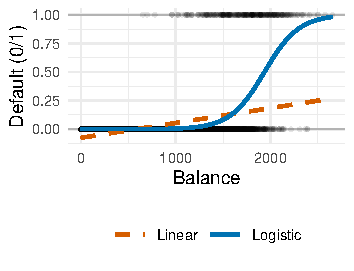
\includegraphics[width=\linewidth,height=6cm,keepaspectratio]{figures/cls_linear_vs_logistic}
            \par{\scriptsize \texttt{Default} data: the linear fit is negative for small balances, the logistic fit stays in $[0, 1]$.}
        \end{column}
    \end{columns}
\end{frame}


\begin{frame}{Measuring Classification Error}
    \begin{itemize}
        \item A classifier's mistakes are counted by the error rate: the fraction of observations whose predicted class differs from the true class.
        \item With predictions $\hat{y}^{(i)}$ for $i = 1, \dots, n$:
        \[
            \text{error rate} = \frac{1}{n} \sum_{i=1}^{n} \mathbb{1}\{y^{(i)} \neq \hat{y}^{(i)}\}.
        \]
        \item The indicator $\mathbb{1}\{A\}$ equals $1$ if the statement $A$ is true and $0$ otherwise, so the sum counts the mistakes. Example: $8$ mistakes among $100$ observations gives an error rate of $0.08$.
        \item Computed on the training data this is the training error rate; what matters is the error on new observations, treated in a later lecture.
    \end{itemize}
\end{frame}


\begin{frame}{Conditional Class Probabilities}
    \begin{itemize}
        \item For a fixed $\mathbf{x}$ the class is still random: customers with identical balance, income and student status do not all default, or all repay.
        \item The conditional class probability $p_k(\mathbf{x}) = P(y = k \mid \mathbf{x})$ is the probability that the response is class $k$ given the feature vector $\mathbf{x}$. Read it as the long-run proportion of observations with exactly this $\mathbf{x}$ that belong to class $k$.
        \item The probabilities of all classes sum to one: $\sum_{k=1}^{K} p_k(\mathbf{x}) = 1$.
        \item Example with $K = 3$ land-cover classes at a pixel with spectral values $\mathbf{x}$: $p_{\text{water}}(\mathbf{x}) = 0.1$, $p_{\text{forest}}(\mathbf{x}) = 0.6$, $p_{\text{urban}}(\mathbf{x}) = 0.3$.
    \end{itemize}
\end{frame}


\begin{frame}{The Bayes Classifier}
    \begin{itemize}
        \item A natural rule: for each $\mathbf{x}$, predict the class with the highest conditional probability.
        \[
            f_{\text{Bayes}}(\mathbf{x}) = \arg\max_{k \in \{1, \dots, K\}} p_k(\mathbf{x}),
        \]
        where $\arg\max$ returns the class $k$ at which $p_k(\mathbf{x})$ is largest.
        \item In the land-cover example the rule predicts forest, since $0.6$ is the largest of the three probabilities.
        \item For two classes with $y \in \{0, 1\}$ and $p(\mathbf{x}) = P(y = 1 \mid \mathbf{x})$: predict $1$ if $p(\mathbf{x}) > 0.5$ and $0$ otherwise.
        \item Among all classifiers, the Bayes classifier makes the fewest mistakes on average.
    \end{itemize}
\end{frame}


% \begin{frame}{The Bayes Error Rate}
%     \begin{itemize}
%         \item Even the best prediction can be wrong: at $\mathbf{x}$ the Bayes classifier errs with probability $1 - \max_k p_k(\mathbf{x})$. In the land-cover example, $1 - 0.6 = 0.4$.
%         \item Averaging over the distribution of feature vectors gives the Bayes error rate:
%         \[
%             1 - \mathbb{E}_{\mathbf{x}}\!\left[\max_k p_k(\mathbf{x})\right].
%         \]
%         \item It is irreducible: classes overlap, so the same $\mathbf{x}$ can come from different classes, and no classifier can avoid these errors.
%         \item It is the benchmark: the error rate of any classifier on new data is at least the Bayes error rate.
%     \end{itemize}
% \end{frame}


% \begin{frame}{Bayes Error Rate: A Small Example}
%     \begin{itemize}
%         \item Binary response and a single feature $x$ taking three values $a$, $b$, $c$, each with probability $1/3$.
%         \item At each value the Bayes classifier predicts the more probable class and errs with probability $1 - \max\{p(x), 1 - p(x)\}$.
%     \end{itemize}
%     \begin{center}
%         {\small
%         \renewcommand{\arraystretch}{1.15}
%         \begin{tabular}{cccc}
%         \toprule
%         $x$ & $p(x) = P(y = 1 \mid x)$ & Bayes prediction & Error probability \\
%         \midrule
%         $a$ & $0.9$ & $1$ & $0.1$ \\
%         $b$ & $0.4$ & $0$ & $0.4$ \\
%         $c$ & $0.2$ & $0$ & $0.2$ \\
%         \bottomrule
%         \end{tabular}
%         }
%     \end{center}
%     \begin{itemize}
%         \item Bayes error rate: $\frac{1}{3}(0.1 + 0.4 + 0.2) \approx 0.23$. The error is largest at $b$, where $p(x)$ is close to $0.5$.
%     \end{itemize}
% \end{frame}


\begin{frame}{From the Bayes Classifier to Practical Classifiers}
    \begin{itemize}
        \item The Bayes classifier is an unattainable gold standard: the true $p_k(\mathbf{x})$ is unknown.
        \item Practical classifiers estimate $\hat{p}_k(\mathbf{x})$ from the training data and plug it into the same rule: predict $\arg\max_k \hat{p}_k(\mathbf{x})$.
        \item Logistic regression estimates $p_k(\mathbf{x})$ with a parametric model whose parameters are fitted by maximum likelihood.
        \item $k$-nearest neighbors estimates $p_k(\mathbf{x})$ with class proportions among nearby training points.
    \end{itemize}
\end{frame}


\begin{frame}{Decision Boundaries}
    \begin{sitemize}
        \item A classifier splits the feature space $\mathbb{R}^p$ into regions $R_k = \{\mathbf{x} : f(\mathbf{x}) = k\}$; the decision boundary is where regions meet.
        \item For two classes, the Bayes decision boundary is $\{\mathbf{x} : p_1(\mathbf{x}) = 0.5\}$.
        \item A linear boundary is a hyperplane, $\symbf{\beta}^\top \tilde{\mathbf{x}} = 0$; a nonlinear boundary is curved.
    \end{sitemize}
    \begin{center}
        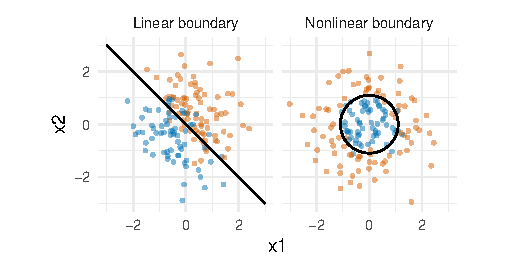
\includegraphics[height=4.5cm]{figures/cls_boundaries_linear_nonlinear}
    \end{center}
\end{frame}


\subsection{Logistic Regression}


\begin{frame}{Modeling a Binary Response}
    \begin{itemize}
        \item Linear regression models the mean of a quantitative response given the features: $\mathbb{E}[y \mid \mathbf{x}] = \symbf{\beta}^\top \tilde{\mathbf{x}}$, with random errors around this mean.
        \item A binary response $y \in \{0, 1\}$ given $\mathbf{x}$ has a Bernoulli distribution: $P(y = 1 \mid \mathbf{x}) = p(\mathbf{x})$ and $P(y = 0 \mid \mathbf{x}) = 1 - p(\mathbf{x})$.
        \item The mean of a Bernoulli variable is its success probability: $\mathbb{E}[y \mid \mathbf{x}] = 1 \cdot p(\mathbf{x}) + 0 \cdot \big(1 - p(\mathbf{x})\big) = p(\mathbf{x})$.
        \item So, as in linear regression, we model how the mean of $y$ depends on $\mathbf{x}$. Here the mean is a probability, so it must stay in $[0, 1]$.
    \end{itemize}
\end{frame}


\begin{frame}{The Logistic Function}
    \begin{itemize}
        \item Keep a linear score $z = \symbf{\beta}^\top \tilde{\mathbf{x}} = \beta_0 + \beta_1 x_1 + \dots + \beta_p x_p$, which can take any real value, and pass it through a function that maps $\mathbb{R}$ to $(0, 1)$: the logistic (sigmoid) function $\sigma(z) = 1 / (1 + e^{-z})$.
        \item The logistic regression model:
        \[
            p(\mathbf{x}) = \sigma(\symbf{\beta}^\top \tilde{\mathbf{x}}) = \frac{1}{1 + e^{-\symbf{\beta}^\top \tilde{\mathbf{x}}}}, \qquad \symbf{\beta} = (\beta_0, \beta_1, \dots, \beta_p)^\top.
        \]
        \item Properties: $\sigma(z) \in (0, 1)$, $\sigma(0) = 0.5$, $\sigma$ is increasing, and $\sigma(-z) = 1 - \sigma(z)$.
        \item Fitted probabilities $\hat{p}(\mathbf{x})$ are therefore always valid, and the fitted curve is S-shaped rather than a straight line.
    \end{itemize}
\end{frame}


\begin{frame}{Odds}
    \begin{itemize}
        \item The odds of an event compare the probability that it happens with the probability that it does not: $\dfrac{p(\mathbf{x})}{1 - p(\mathbf{x})} \in (0, \infty)$.
        \item Examples: $p = 0.8$ gives odds of $4$ (four to one in favour of $y = 1$), $p = 0.5$ gives odds of $1$ (even odds), $p = 0.2$ gives odds of $0.25$.
        \item Odds above $1$ mean $y = 1$ is more likely than $y = 0$; odds below $1$ mean it is less likely.
    \end{itemize}
\end{frame}


\begin{frame}{Log-Odds}
    \begin{itemize}
        \item The log-odds, or logit, $\log \dfrac{p(\mathbf{x})}{1 - p(\mathbf{x})} \in (-\infty, \infty)$, removes the lower bound of the odds.
        \item It is symmetric around $p = 0.5$, where the log-odds equal $0$.
        \item The logit is the inverse of the logistic function.
    \end{itemize}
    \begin{center}
        {\small
        \renewcommand{\arraystretch}{1.15}
        \begin{tabular}{lccccc}
        \toprule
        probability $p$ & $0.1$ & $0.2$ & $0.5$ & $0.8$ & $0.9$ \\
        odds & $0.11$ & $0.25$ & $1$ & $4$ & $9$ \\
        log-odds & $-2.20$ & $-1.39$ & $0$ & $1.39$ & $2.20$ \\
        \bottomrule
        \end{tabular}
        }
    \end{center}
\end{frame}


\begin{frame}{Logistic Regression Is Linear in the Log-Odds}
    \begin{itemize}
        \item With $z = \symbf{\beta}^\top \tilde{\mathbf{x}}$ and $p(\mathbf{x}) = 1 / (1 + e^{-z})$, we have $1 - p(\mathbf{x}) = e^{-z} / (1 + e^{-z})$, so
        \[
            \frac{p(\mathbf{x})}{1 - p(\mathbf{x})} = \frac{1}{e^{-z}} = e^{z}.
        \]
        \item Taking logs, the log-odds is linear in $\mathbf{x}$:
        \[
            \log \frac{p(\mathbf{x})}{1 - p(\mathbf{x})} = \symbf{\beta}^\top \tilde{\mathbf{x}}.
        \]
        \item Logistic regression is therefore a linear regression for the log-odds: the logit connects the mean of $y$ (a probability) to the linear score, the same idea as regression on a different scale.
    \end{itemize}
\end{frame}


\begin{frame}{Interpreting the Coefficients}
    \begin{itemize}
        \item Increasing $x_j$ by one unit with the other features fixed adds $\beta_j$ to the log-odds, i.e.\ multiplies the odds by $e^{\beta_j}$ (an odds ratio).
        \item If $\beta_j > 0$ the probability of $y = 1$ increases with $x_j$; if $\beta_j < 0$ it decreases; if $\beta_j = 0$ there is no association.
        \item The change in $p(\mathbf{x})$ itself is not constant: doubling the odds moves $p$ from $0.10$ to $0.18$, from $0.50$ to $0.67$, and from $0.90$ to $0.95$.
        \item Coefficients are therefore interpreted on the log-odds or odds scale, not as changes in probability.
    \end{itemize}
\end{frame}


\begin{frame}{Estimation: The Likelihood Idea}
    \begin{itemize}
        \item Least squares is built for a quantitative response with additive errors; for a Bernoulli response we use a different principle, maximum likelihood.
        \item Idea: choose the parameter values under which the observed data would have been most probable.
        \item The likelihood is the probability of the observed data, viewed as a function of the parameters with the data held fixed.
        \item The maximum likelihood estimate is the parameter value that maximizes the likelihood.
    \end{itemize}
\end{frame}


\begin{frame}{Likelihood: A Coin-Flip Example}
    \begin{itemize}
        \item A coin lands heads with unknown probability $\theta$. We flip it $10$ times and observe a particular sequence with $7$ heads and $3$ tails.
        \item The flips are independent, so the probability of this sequence is the likelihood $L(\theta) = \theta^{7} (1 - \theta)^{3}$.
        \item Comparing values: $L(0.5) \approx 0.00098$ and $L(0.7) \approx 0.00222$. The data are more than twice as probable under $\theta = 0.7$.
        \item The likelihood is maximized at $\hat{\theta} = 7/10$, the observed proportion of heads: maximum likelihood agrees with intuition.
    \end{itemize}
    \dual{}{
        \paragraph{Maximizing the coin-flip likelihood.}
        Since the logarithm is increasing (see below), we may maximize $\log L(\theta) = 7 \log \theta + 3 \log (1 - \theta)$ instead. Setting the derivative to zero,
        \[
            \frac{7}{\theta} - \frac{3}{1 - \theta} = 0 \quad \Longrightarrow \quad \hat{\theta} = \frac{7}{10}.
        \]
        With $m$ heads in $n$ flips the same steps give $\hat{\theta} = m / n$.
    }
\end{frame}


\begin{frame}{Bernoulli Likelihood of One Observation}
    \begin{itemize}
        \item Given $\mathbf{x}^{(i)}$, the label is Bernoulli, $y^{(i)} \mid \mathbf{x}^{(i)} \sim \text{Bernoulli}(p^{(i)})$. The probability of the observed label has a single formula:
        \[
            P\big(y^{(i)} \mid \mathbf{x}^{(i)}\big) = \big(p^{(i)}\big)^{y^{(i)}} \big(1 - p^{(i)}\big)^{1 - y^{(i)}}.
        \]
        \item It equals $p^{(i)}$ when $y^{(i)} = 1$ and $1 - p^{(i)}$ when $y^{(i)} = 0$.
        \item The regression model enters through the success probability: $p^{(i)} = p(\mathbf{x}^{(i)}) = \sigma(\symbf{\beta}^\top \tilde{\mathbf{x}}^{(i)})$.
        \item So the probability the model assigns to each observed label depends on the parameter vector $\symbf{\beta}$.
    \end{itemize}
\end{frame}


\begin{frame}{Likelihood of the Sample}
    \begin{itemize}
        \item The observations are independent, so the probability of all $n$ labels is the product of the individual probabilities:
        \[
            \begin{aligned}
                L(\symbf{\beta}) &= \prod_{i=1}^{n} \big(p^{(i)}\big)^{y^{(i)}} \big(1 - p^{(i)}\big)^{1 - y^{(i)}} \\
                &= \prod_{i : y^{(i)} = 1} p^{(i)} \prod_{i : y^{(i)} = 0} \big(1 - p^{(i)}\big).
            \end{aligned}
        \]
        \item $L$ is large when $p^{(i)}$ is close to $1$ for observations with $y^{(i)} = 1$ and close to $0$ for observations with $y^{(i)} = 0$, i.e.\ when the coefficients fit the observed labels well.
        \item The maximum likelihood estimates are $\hat{\symbf{\beta}} = \arg\max_{\symbf{\beta}} L(\symbf{\beta})$.
    \end{itemize}
\end{frame}


\begin{frame}{Why the Log-Likelihood?}
    \begin{itemize}
        \item A product of $n$ probabilities, each below $1$, is extremely small and numerically unstable: $0.9^{1000} \approx 10^{-46}$.
        \item The logarithm is strictly increasing, so $L$ and $\log L$ are maximized by the same parameter values.
        \item The logarithm turns the product into a sum, with one simple term per observation:
        \[
            \ell(\symbf{\beta}) = \log L = \sum_{i=1}^{n} \Big[ y^{(i)} \log p^{(i)} + \big(1 - y^{(i)}\big) \log \big(1 - p^{(i)}\big) \Big].
        \]
        \item Sums are far easier to differentiate than products.
    \end{itemize}
\end{frame}


\begin{frame}{Why Maximize?}
    \begin{itemize}
        \item $L$ is the probability the model assigns to the data we actually observed: a larger value means the parameters explain the data better. It is not the probability that the parameters are correct.
        \item Each term of $\ell$ is the logarithm of a probability, hence at most $0$; the best fit gives the value of $\ell$ closest to $0$.
        \item For one observation with $y^{(i)} = 1$ the term is $\log p^{(i)}$: near $0$ when $p^{(i)}$ is near $1$, and tending to $-\infty$ as $p^{(i)} \to 0$. Confident wrong predictions are penalized heavily.
        \item Machine learning usually minimizes a loss: maximizing $\ell$ is the same as minimizing the cross-entropy loss $-\ell / n$.
    \end{itemize}
\end{frame}


\begin{frame}{Maximizing the Log-Likelihood}
    \begin{itemize}
        \item Stack the labels and the fitted probabilities into $\mathbf{y} = (y^{(i)})_{i=1}^n$ and $\mathbf{p} = (p^{(i)})_{i=1}^n$, where $p^{(i)} = \sigma(\symbf{\beta}^\top \tilde{\mathbf{x}}^{(i)})$.
        \item The gradient of the log-likelihood is $\nabla \ell(\symbf{\beta}) = \tilde{\mathbf{X}}^\top (\mathbf{y} - \mathbf{p})$.
        \item Setting it to zero gives the score equations $\tilde{\mathbf{X}}^\top (\mathbf{y} - \mathbf{p}) = \mathbf{0}$. They resemble the normal equations of least squares, but $\mathbf{p}$ is nonlinear in $\symbf{\beta}$, so there is no closed-form solution.
        \item $\ell$ is concave, so any solution is a global maximum. It is found iteratively by Newton--Raphson (IRLS), which is what \texttt{glm()} in R uses.
    \end{itemize}
    \dual{}{
        \paragraph{Derivation of the gradient and the Newton step.}
        Let $z^{(i)} = \symbf{\beta}^\top \tilde{\mathbf{x}}^{(i)}$, so $p^{(i)} = \sigma(z^{(i)})$ and $\sigma'(z) = \sigma(z)\big(1 - \sigma(z)\big)$. The contribution of observation $i$ to $\ell$ is $\ell^{(i)} = y^{(i)} \log p^{(i)} + (1 - y^{(i)}) \log (1 - p^{(i)})$, and
        \[
            \frac{\partial \ell^{(i)}}{\partial z^{(i)}} = \Big( \frac{y^{(i)}}{p^{(i)}} - \frac{1 - y^{(i)}}{1 - p^{(i)}} \Big) p^{(i)} \big(1 - p^{(i)}\big) = y^{(i)} - p^{(i)}.
        \]
        By the chain rule, $\partial \ell^{(i)} / \partial \symbf{\beta} = (y^{(i)} - p^{(i)}) \tilde{\mathbf{x}}^{(i)}$, and summing over $i$ gives $\nabla \ell(\symbf{\beta}) = \tilde{\mathbf{X}}^\top (\mathbf{y} - \mathbf{p})$. Differentiating once more gives the Hessian $-\tilde{\mathbf{X}}^\top \mathbf{W} \tilde{\mathbf{X}}$ with $\mathbf{W} = \operatorname{diag}\big(p^{(i)} (1 - p^{(i)})\big)$, which is negative definite when $\tilde{\mathbf{X}}$ has full column rank, so $\ell$ is strictly concave. Newton--Raphson therefore iterates
        \[
            \symbf{\beta}^{\text{new}} = \symbf{\beta} + \big( \tilde{\mathbf{X}}^\top \mathbf{W} \tilde{\mathbf{X}} \big)^{-1} \tilde{\mathbf{X}}^\top (\mathbf{y} - \mathbf{p}),
        \]
        which equals a weighted least-squares fit with weights $\mathbf{W}$ and working response $\tilde{\mathbf{X}} \symbf{\beta} + \mathbf{W}^{-1} (\mathbf{y} - \mathbf{p})$; this is why the algorithm is called iteratively reweighted least squares (IRLS).
    }
\end{frame}


\begin{frame}{Making Predictions}
    \begin{itemize}
        \item For a new observation $\mathbf{x}^\ast$, the fitted probability is $\hat{p}(\mathbf{x}^\ast) = \sigma(\hat{\symbf{\beta}}^\top \tilde{\mathbf{x}}^\ast)$.
        \item Classify with a threshold $\tau$: predict $\hat{y}^\ast = 1$ if $\hat{p}(\mathbf{x}^\ast) > \tau$, else $\hat{y}^\ast = 0$.
        \item The default $\tau = 0.5$ is the Bayes rule with the estimated probability in place of the true one.
        \item A lower $\tau$ labels more observations as class $1$ (for example, flags more customers as likely defaulters); the trade-off between the two kinds of error is treated in a later lecture.
    \end{itemize}
\end{frame}


\begin{frame}{The Logistic Decision Boundary}
    \begin{columns}[T]
        \begin{column}{0.56\textwidth}
            \begin{itemize}
                \item For $\tau = 0.5$, $\hat{y}^\ast = 1 \iff \hat{\symbf{\beta}}^\top \tilde{\mathbf{x}}^\ast > 0$ (since $\sigma(z) > 0.5 \iff z > 0$), so the boundary $\hat{\symbf{\beta}}^\top \tilde{\mathbf{x}} = 0$ is a hyperplane.
                \item Logistic regression is a linear classifier, although $p(\mathbf{x})$ is nonlinear in $\mathbf{x}$.
                \item Another $\tau$ gives $\hat{\symbf{\beta}}^\top \tilde{\mathbf{x}} = \log \frac{\tau}{1 - \tau}$, a parallel hyperplane.
            \end{itemize}
        \end{column}
        \begin{column}{0.44\textwidth}
            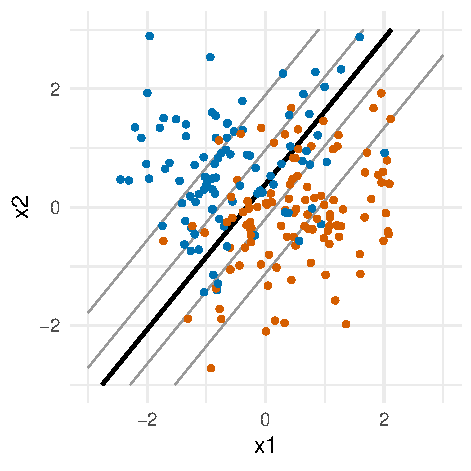
\includegraphics[width=\linewidth,height=8cm,keepaspectratio]{figures/cls_logistic_boundary}
            \par{\scriptsize Black: $\hat{p} = 0.5$; grey: $0.1, 0.3, 0.7, 0.9$.}
        \end{column}
    \end{columns}
\end{frame}


\begin{frame}{Worked Example: Default Data}
    \begin{itemize}
        \item \texttt{Default}: $10{,}000$ credit card customers, response \texttt{default} ($333$ defaults), predictors \texttt{balance}, \texttt{income}, \texttt{student}.
        \item Fit: \texttt{glm(default \textasciitilde{} balance, data = Default, family = binomial)}.
    \end{itemize}
    \begin{center}
        {\small
        \renewcommand{\arraystretch}{1.15}
        \begin{tabular}{lrrrr}
        \toprule
        & Estimate & Std.\ error & $z$ & $p$-value \\
        \midrule
        Intercept & $-10.6513$ & $0.3612$ & $-29.49$ & $< 2 \times 10^{-16}$ \\
        \texttt{balance} & $0.00550$ & $0.00022$ & $24.95$ & $< 2 \times 10^{-16}$ \\
        \bottomrule
        \end{tabular}
        }
    \end{center}
\end{frame}


\begin{frame}{Interpreting the Default Fit}
    \begin{itemize}
        \item $e^{100 \hat{\beta}_1} \approx 1.73$: each additional \$100 of balance multiplies the odds of default by about $1.73$ (95\% CI $[1.66, 1.81]$).
        \item The coefficient of \texttt{balance} is positive and highly significant ($z = 24.95$): higher balances go with a higher probability of default.
        \item The intercept is the log-odds of default at zero balance: $\hat{p}(\text{balance} = 0) \approx 0.00002$.
        \item Predictions: $\hat{p}(1000) = \sigma(-10.6513 + 0.00550 \times 1000) \approx 0.006$ and $\hat{p}(2000) \approx 0.586$.
    \end{itemize}
\end{frame}


\begin{frame}{Multiple Logistic Regression}
    \begin{itemize}
        \item Additional predictors enter the log-odds linearly:
        \[
            \log \frac{p(\mathbf{x})}{1 - p(\mathbf{x})} = \beta_0 + \beta_1 x_1 + \dots + \beta_p x_p = \symbf{\beta}^\top \tilde{\mathbf{x}}.
        \]
        \item Each $\beta_j$ is the effect of $x_j$ on the log-odds holding the other predictors fixed, and $e^{\beta_j}$ is the corresponding odds ratio.
        \item A categorical predictor enters through dummy variables, for example $x = 1$ for a student and $x = 0$ otherwise.
    \end{itemize}
\end{frame}


\begin{frame}{Confounding: Student Status in the Default Data}
    \begin{itemize}
        \item With student as the only predictor, its coefficient is $+0.405$ ($p < 0.001$): students default more often.
        \item With balance and income included, it is $-0.647$ ($p = 0.006$): a student defaults less often than a non-student with the same balance and income.
        \item Students carry higher balances on average (about \$988 vs.\ \$772), and higher balances raise default risk.
        \item As in multiple linear regression, the marginal and the conditional effect can differ in sign.
    \end{itemize}
\end{frame}


\begin{frame}{Multinomial Regression}
    \begin{itemize}
        \item For $K > 2$ classes, model every class probability with the softmax function:
        \[
            P(y = k \mid \mathbf{x}) = \frac{\exp(\symbf{\beta}_k^\top \tilde{\mathbf{x}})}{\sum_{l=1}^{K} \exp(\symbf{\beta}_l^\top \tilde{\mathbf{x}})}, \qquad k = 1, \dots, K.
        \]
        \item Each class has its own coefficient vector $\symbf{\beta}_k = (\beta_{k0}, \beta_{k1}, \dots, \beta_{kp})^\top$, including an intercept. The probabilities are positive and sum to one.
        \item Boundaries between any pair of classes remain linear in $\mathbf{x}$, since $P(y = k \mid \mathbf{x}) = P(y = l \mid \mathbf{x})$ reduces to $\symbf{\beta}_k^\top \tilde{\mathbf{x}} = \symbf{\beta}_l^\top \tilde{\mathbf{x}}$.
    \end{itemize}
\end{frame}


\begin{frame}{Identifiability and the Reference Class}
    \begin{itemize}
        \item A model is identifiable if distinct parameter values always give distinct probabilities. Otherwise the data cannot single out one estimate, and the likelihood has no unique maximizer.
        \item The softmax model is not identifiable: adding the same vector $\mathbf{c} \in \mathbb{R}^{p+1}$ to every $\symbf{\beta}_k$ multiplies the numerator and every term of the denominator by $e^{\mathbf{c}^\top \tilde{\mathbf{x}}}$. The factor cancels and all $K$ probabilities are unchanged.
        \item Fix a reference class, usually $K$, by setting $\symbf{\beta}_K = \mathbf{0}$. Exactly one parameter set in each group of equivalent sets satisfies this.
        \item The remaining $K - 1$ classes each have $p + 1$ free parameters.
    \end{itemize}
\end{frame}


\begin{frame}{Interpreting Multinomial Coefficients}
    \begin{itemize}
        \item Relative to the reference class,
        \[
            \log \frac{P(y = k \mid \mathbf{x})}{P(y = K \mid \mathbf{x})} = \symbf{\beta}_k^\top \tilde{\mathbf{x}}, \qquad k = 1, \dots, K - 1.
        \]
        \item So $\beta_{kj}$ is the change in the log-odds of class $k$ versus class $K$ per unit increase in $x_j$ with the other features fixed, and $e^{\beta_{kj}}$ multiplies the odds of class $k$ relative to class $K$.
        \item The coefficients depend on the choice of reference class; the fitted probabilities do not.
        \item For $K = 2$ with class $2$ as the reference, $P(y = 1 \mid \mathbf{x}) = \sigma(\symbf{\beta}_1^\top \tilde{\mathbf{x}})$: ordinary logistic regression.
    \end{itemize}
\end{frame}


\begin{frame}{Nonlinear Decision Boundaries}
    \begin{itemize}
        \item Add transformed features such as $x_1^2$, $x_2^2$, $x_1 x_2$ to the linear score; the model stays linear in the parameters, exactly as in polynomial regression.
        \item Example:
        \[
            \log \frac{p(\mathbf{x})}{1 - p(\mathbf{x})} = \beta_0 + \beta_1 x_1^2 + \beta_2 x_2^2.
        \]
        \item If $\beta_1 = \beta_2$ and $\beta_0$ has the opposite sign, the boundary is the circle $x_1^2 + x_2^2 = r^2$ with $r^2 = -\beta_0 / \beta_1$, which is a linear boundary in the features $(x_1^2, x_2^2)$.
    \end{itemize}
\end{frame}


\begin{frame}{Feature Maps and Overfitting}
    \begin{itemize}
        \item More generally, replace $\mathbf{x}$ with a feature map $\phi(\mathbf{x})$ and fit logistic regression on $\phi(\mathbf{x})$: the boundary is linear in $\phi(\mathbf{x})$-space and nonlinear in $\mathbf{x}$-space.
        \item The likelihood, the fitting algorithm and the interpretation of coefficients carry over unchanged.
        \item A richer feature map fits the training boundary more closely but risks overfitting; how many terms to add is the same trade-off as choosing the polynomial degree.
    \end{itemize}
\end{frame}


\subsection{\texorpdfstring{$k$}{k}-Nearest Neighbors}


\begin{frame}{\texorpdfstring{$k$}{k}-Nearest Neighbors Classifier}
    \begin{itemize}
        \item $k$-NN is nonparametric: there is no model to fit, and predictions use the training data directly.
        \item For a new point $\mathbf{x}^\ast$ and a chosen integer $k$, let $\mathcal{N}^\ast$ be the set of indices of the $k$ training points closest to $\mathbf{x}^\ast$.
        \item Estimate the class probabilities by the class proportions in the neighbourhood:
        \[
            \hat{p}_j(\mathbf{x}^\ast) = \frac{1}{k} \sum_{i \in \mathcal{N}^\ast} \mathbb{1}\{y^{(i)} = j\}.
        \]
    \end{itemize}
\end{frame}


\begin{frame}{\texorpdfstring{$k$}{k}-NN: Majority Vote}
    \begin{itemize}
        \item Classify by majority vote, $\hat{y}^\ast = \arg\max_j \hat{p}_j(\mathbf{x}^\ast)$: the Bayes rule applied to the estimated probabilities.
        \item Ties are broken at random.
        \item Example: with $k = 3$ and two of the three nearest neighbours in class $1$, $\hat{p}_1(\mathbf{x}^\ast) = 2/3$ and $\hat{y}^\ast = 1$.
    \end{itemize}
\end{frame}


\begin{frame}{Distance Metrics}
    \begin{itemize}
        \item ``Closest'' requires a distance, and different distances can give different neighbours.
        \item The default is Euclidean, $d(\mathbf{a}, \mathbf{b}) = \lVert \mathbf{a} - \mathbf{b} \rVert_2 = \sqrt{\sum_{j=1}^{p} (a_j - b_j)^2}$.
        \item Alternatives: Manhattan, $\sum_{j=1}^{p} |a_j - b_j|$, and the Minkowski family $\big( \sum_{j=1}^{p} |a_j - b_j|^q \big)^{1/q}$, which contains both ($q = 1$ and $q = 2$).
    \end{itemize}
\end{frame}


\begin{frame}{Feature Scaling}
    \begin{itemize}
        \item Features with a large spread dominate the distance: in \texttt{Default}, \texttt{income} has a standard deviation of about \$13{,}300 and \texttt{balance} about \$480, so raw distances are driven almost entirely by \texttt{income}, the weaker predictor of default.
        \item Standardize before computing distances, $z_j^{(i)} = (x_j^{(i)} - \bar{x}_j) / s_j$, where $\bar{x}_j$ and $s_j$ are the sample mean and standard deviation of feature $j$.
        \item Every standardized feature has mean $0$ and standard deviation $1$, so all features contribute on a comparable scale.
        \item Preprocessing is treated in detail in a later lecture.
    \end{itemize}
\end{frame}


\begin{frame}{The Effect of \texorpdfstring{$k$}{k}}
    \begin{itemize}
        \item Small $k$ ($k = 1$): jagged boundary following individual points; training error is $0$, which says nothing about new data.
        \item Large $k$: smooth, rigid boundary that can miss genuine curvature; $k = n$ predicts the majority class everywhere.
        \item $k$ is a tuning parameter; choosing it needs held-out data (a later lecture).
    \end{itemize}
    \begin{center}
        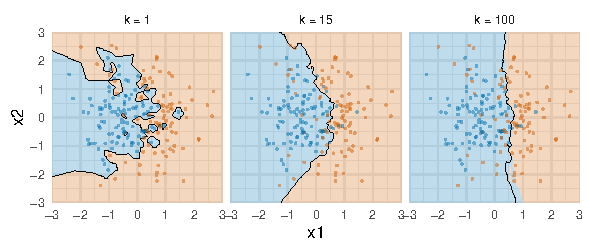
\includegraphics[height=4.25cm]{figures/cls_knn_k}
    \end{center}
\end{frame}


\begin{frame}{\texorpdfstring{$k$}{k}-NN: Strengths}
    \begin{itemize}
        \item No fitting step: predictions use the stored training data directly.
        \item No assumption about the shape of the decision boundary.
        \item A single tuning parameter $k$, and easy to explain.
    \end{itemize}
\end{frame}


\begin{frame}{\texorpdfstring{$k$}{k}-NN: Weaknesses}
    \begin{itemize}
        \item Cost: every prediction computes distances to all $n$ training points, $O(np)$ per query, and the whole training set must be stored.
        \item Curse of dimensionality: as $p$ grows the data become sparse and the ``nearest'' neighbours are no longer near; irrelevant features add noise to every distance.
        \item No coefficients: $k$-NN gives predictions but no summary of how each feature affects the outcome, unlike $e^{\beta_j}$ in logistic regression.
        \item Sensitive to feature scaling.
    \end{itemize}
\end{frame}


\subsection{Comparison and Summary}


\begin{frame}{Logistic Regression vs.\ \texorpdfstring{$k$}{k}-NN on the Same Data}
    \begin{columns}[T]
        \begin{column}{0.48\textwidth}
            \begin{itemize}
                \item Same simulated data (curved true boundary); boundaries drawn at $\hat{p} = 0.5$.
                \item Logistic regression: a straight line, misses the curvature.
                \item $k$-NN ($k = 15$): follows the curve, locally jagged.
                \item Which is better depends on the true boundary and the sample size; judging it needs held-out data.
            \end{itemize}
        \end{column}
        \begin{column}{0.52\textwidth}
            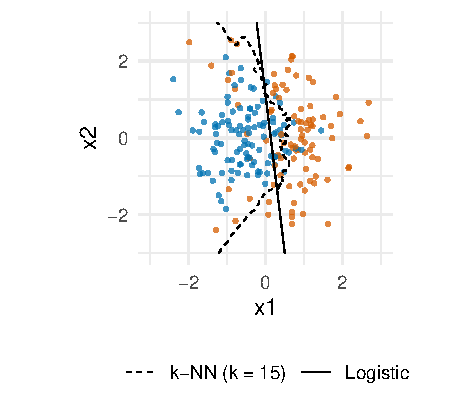
\includegraphics[width=\linewidth,height=8cm,keepaspectratio]{figures/cls_logistic_vs_knn}
        \end{column}
    \end{columns}
\end{frame}


\begin{frame}{Logistic Regression vs.\ \texorpdfstring{$k$}{k}-NN}
    \begin{center}
        {\small
        \renewcommand{\arraystretch}{1.25}
        \begin{tabular}{@{}lp{0.33\textwidth}p{0.33\textwidth}@{}}
        \toprule
        & Logistic regression & $k$-NN \\
        \midrule
        Type & Parametric: $\symbf{\beta}$ & Nonparametric: stores the training data \\
        Decision boundary & Linear, unless features are added & Flexible, controlled by $k$ \\
        Fitting & Iterative maximum likelihood & None \\
        Cost per prediction & $O(p)$ & $O(np)$ \\
        Interpretation & Odds ratios $e^{\beta_j}$, $z$-tests, confidence intervals & No coefficients \\
        Main weakness & Misses nonlinear structure unless features are engineered & Feature scaling, irrelevant features, high dimensions \\
        \bottomrule
        \end{tabular}
        }
    \end{center}
\end{frame}


\begin{frame}{Summary: Classification and Logistic Regression}
    \begin{itemize}
        \item Classification predicts a category by estimating the class probabilities $p_k(\mathbf{x})$. The Bayes classifier (most probable class) is the unattainable benchmark, and the Bayes error rate is irreducible.
        \item Logistic regression models the Bernoulli success probability through the log-odds, $\log \frac{p(\mathbf{x})}{1 - p(\mathbf{x})} = \symbf{\beta}^\top \tilde{\mathbf{x}}$; coefficients are read as odds ratios $e^{\beta_j}$.
        \item The coefficients maximize the likelihood, equivalently the log-likelihood or minus the cross-entropy, found iteratively; the decision boundary is linear.
        \item It extends to $K > 2$ classes through the multinomial model with a reference class, and to nonlinear boundaries through added features.
    \end{itemize}
\end{frame}


\begin{frame}{Summary: \texorpdfstring{$k$}{k}-NN and Next Steps}
    \begin{itemize}
        \item $k$-NN: majority vote among the $k$ closest training points, a flexible boundary controlled by $k$; it needs feature scaling and degrades in high dimensions.
        \item Logistic regression is parametric, interpretable and linear; $k$-NN is nonparametric and flexible but has no coefficients.
        \item Still open: how to choose $k$ and how to compare classifiers on data not used for fitting.
    \end{itemize}
\end{frame}